\documentclass[14pt,aspectratio=1610]{beamer}

\usepackage[brazil]{babel}
\usepackage[utf8]{inputenc}
%\UseRawInputEncoding
\usepackage[T1]{fontenc}
%\usepackage{Sweave}
\usepackage{animate}
\usepackage{amsbsy}
\usepackage{amsfonts}
\usepackage{amsmath}
\usepackage{amssymb}
\usepackage{amsthm}
\usepackage[toc,page,title,titletoc]{appendix}
%\usepackage[fixlanguage]{babelbib}
%\usepackage[pdftex]{color}
\usepackage{dsfont}
\usepackage{esvect}
\usepackage[labelfont=bf]{caption}
\usepackage{subcaption}
\usepackage{float}
\usepackage[Glenn]{fncychap}%Sonny %Conny %Lenny %Glenn %Renje %Bjarne %Bjornstrup
%\usepackage{geometry, calc, color, setspace}%
%\geometry{a4paper, headsep=1.0cm, footskip=1cm, lmargin=3cm, rmargin=2cm, tmargin=3cm, bmargin=2cm}
\usepackage{graphicx}
\usepackage{indentfirst}%Para indentar os parágrafos automáticamente
\usepackage{lipsum}
\usepackage{longtable}
\usepackage{mathtools}
\usepackage{listings}%Inserir codigo do R no latex
\usepackage{slashbox}
\usepackage{multirow}
\usepackage{multicol}
\usepackage{natbib}
\setcitestyle{authoryear,open={(},close={)}} %Citation-related commands
\bibliographystyle{abbrvnat}
%\usepackage{csquotes}
%\usepackage[natbib=true,style=abnt, sorting=none]{biblatex}
%\addbibresource{bibliografia.bib}
\usepackage[figuresright]{rotating}
\usepackage{spalign}
%\usepackage{pgfpages}
\usepackage{pgfplots}
\pgfplotsset{compat=1.18}
\usepackage{tikz}
\usepackage{color, colortbl}
\usepackage{ragged2e}%para justificar o texto dentro de algum ambiente
\definecolor{Gray}{gray}{0.9}
\definecolor{LightCyan}{rgb}{0.88,1,1}
\definecolor{Lightblue}{RGB}{50, 149, 168}
%\usepackage{grffile}

\usepackage[all]{xy}



\usetheme{Madrid}
\usecolortheme[RGB={193,0,0}]{structure}

%\setbeamertemplate{footline}[frame number]
%\setbeamertemplate{footline}[text line]{%
%  \parbox{\linewidth}{\vspace*{-8pt}\hfill\date{}\hfill\insertshortauthor\hfill\insertpagenumber}}
\beamertemplatenavigationsymbolsempty
\renewcommand{\vec}[1]{\mbox{\boldmath$#1$}}
\newtheorem{Teorema}{Teorema}
\newtheorem{Proposicao}{Proposição}
\newtheorem{Definicao}{Definição}
\newtheorem{Corolario}{Corolário}
\newtheorem{Demonstracao}{Demonstração}
\newcommand{\bx}{\ensuremath{\bar{x}}}
\newcommand{\Ho}{\ensuremath{H_{0}}}
\newcommand{\Hi}{\ensuremath{H_{1}}}
\everymath{\displaystyle}

\apptocmd{\frame}{}{\justifying}{} % Allow optional arguments after frame.

\title{Iniciação à Estatística}
\author{Prof. Fernando de Souza Bastos \texorpdfstring{\\ fernando.bastos@ufv.br}{}}
\institute{Departamento de Estatística \texorpdfstring{\\ Universidade Federal de Viçosa}{}\texorpdfstring{\\ Campus UFV - Viçosa}{}}
\date{}
\newcommand\mytext{Aula 10}
\newcommand\mytextt{Fernando de Souza Bastos}
\newcommand\mytexttt{\url{https://maf105.github.io/}}

\makeatletter
\setbeamertemplate{footline}
{
  \leavevmode%
  \hbox{%
  \begin{beamercolorbox}[wd=.3\paperwidth,ht=2.25ex,dp=1ex,center]{author in head/foot}%
    \usebeamerfont{author in head/foot}\mytext
  \end{beamercolorbox}%
  \begin{beamercolorbox}[wd=.3\paperwidth,ht=2.25ex,dp=1ex,center]{title in head/foot}%
    \usebeamerfont{title in head/foot}\mytextt
  \end{beamercolorbox}%
  \begin{beamercolorbox}[wd=.35\paperwidth,ht=2.25ex,dp=1ex,right]{site in head/foot}%
    \usebeamerfont{site in head/foot}\mytexttt\hspace*{2em}
    \insertframenumber{} / \inserttotalframenumber\hspace*{2ex} 
  \end{beamercolorbox}}%
  \vskip0pt%
}
\makeatother

\providecommand{\arcsin}{} \renewcommand{\arcsin}{\hspace{2pt}\textrm{arcsen}}
\providecommand{\sin}{} \renewcommand{\sin}{\hspace{2pt}\textrm{sen}}
%\newtheorem{Teorema}{Teorema}
%\newtheorem{Proposicao}{Proposição}
%\newtheorem{Definicao}{Definição}
%\newtheorem{Corolario}{Corolário}
%\newtheorem{Demonstracao}{Demonstração}

\titlegraphic{\hspace*{8cm}\href{https://fsbmat-ufv.github.io/}{
\includegraphics[width=2cm]{figs/mylogo.png}}
}


\usepackage{hyperref,bookmark}
\hypersetup{
  colorlinks=true,
  linkcolor=blue,
  citecolor=red,
  filecolor=blue,
  urlcolor=blue,
}

% Layout da pagina
\hypersetup{pdfpagelayout=SinglePage}
\begin{document}
%\Sconcordance{concordance:Aula10.tex:Aula10.Rnw:%
1 167 1 1 15 1 4 34 1 1 15 1 4 18 1 1 13 1 3 5 1 1 13 1 3 5 1 1 13 1 3 %
5 1 1 13 1 3 169 1}


\frame{\titlepage}

\begin{frame}{}
\frametitle{\bf Sumário}
\tableofcontents
\end{frame}

\section{Associação entre Variáveis Quantitativas}
\begin{frame}[fragile]{}
\frametitle{}
\vspace{-0.5cm}
\begin{tabular}{cl}  
        \begin{tabular}{c}
          \parbox{0.5\linewidth}{
          \begin{table}[h!]
  \caption{Anos de Serviço $(X)$ versus\\ N$^{\circ}$ de Clientes $(Y)$}
  \begin{tabular}{ccc}
  \hline
  Agente&X&Y\\
  \hline
  A&2&48\\
  B&4&56\\
  C&5&64\\
  D&6&60\\
  E&6&65\\
  F&6&63\\
  G&7&67\\
  H&8&70\\
  I&8&71\\
  J&10&72\\
  \hline
  \hline
  \end{tabular}
  \end{table}
          }
        \end{tabular}
           & 
        \begin{tabular}{l}
          \setkeys{Gin}{width=0.4\linewidth}
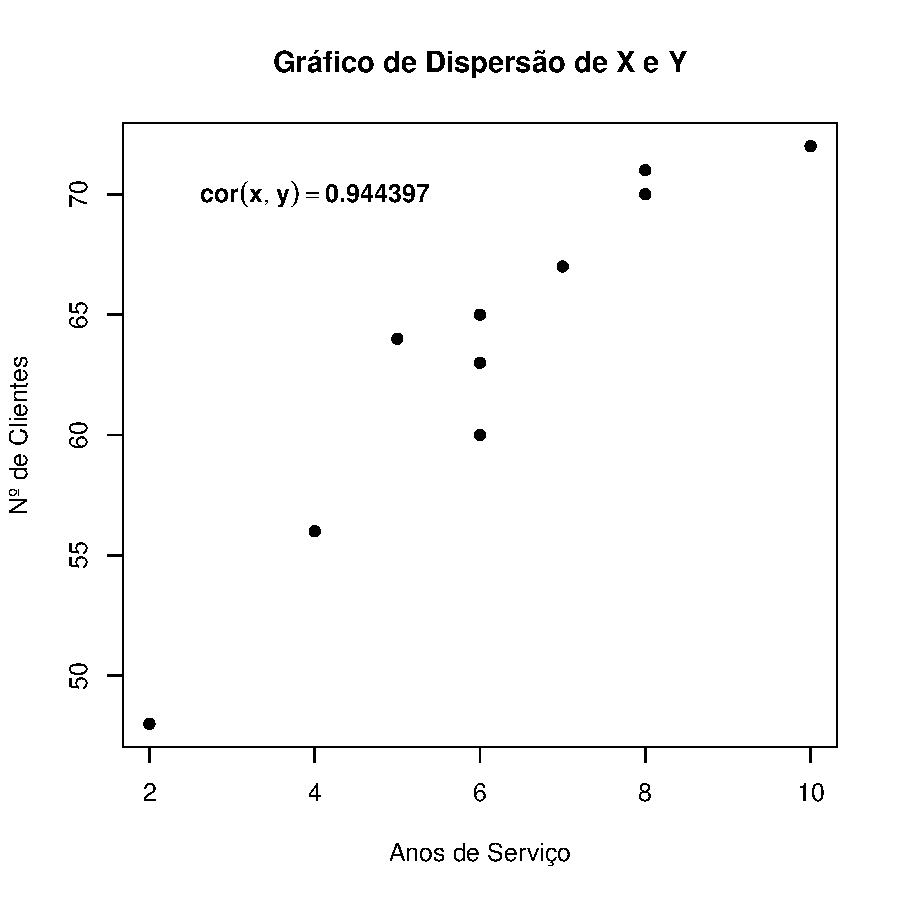
\includegraphics{Aula10-001}
         \end{tabular}  \\
\end{tabular}
\end{frame}

\begin{frame}[fragile]{}
\frametitle{}
\vspace{-0.5cm}
\begin{tabular}{cl}  
        \begin{tabular}{c}
          \parbox{0.5\linewidth}{
          \begin{table}[h!]
  \caption{Renda bruta mensal $(X)$ e porcentagem da renda gasta em saúde $(Y).$}
  \begin{tabular}{ccc}
  \hline
  Família&X&Y\\
  \hline
  A&12&7.2\\
  B&16&7.4\\
  C&18&7.0\\
  D&20&6.5\\
  E&28&6.6\\
  F&30&6.7\\
  G&40&6.0\\
  H&48&5.6\\
  I&50&6.0\\
  J&54&5.5\\
  \hline
  \hline
  \end{tabular}
  \end{table}
          }
        \end{tabular}
           & 
        \begin{tabular}{l}
          \setkeys{Gin}{width=0.4\linewidth}
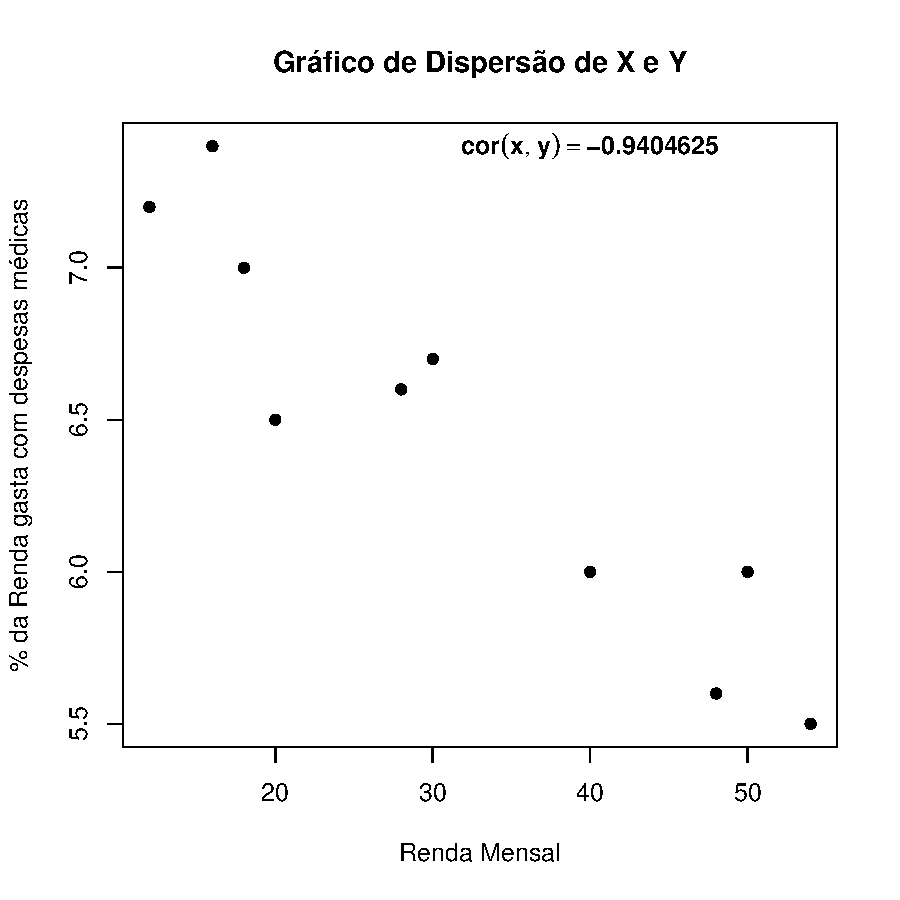
\includegraphics{Aula10-002}
         \end{tabular}  \\
\end{tabular}
\end{frame}

\begin{frame}{}
\frametitle{}
\begin{block}{}
\begin{figure}[H]
    \centering
    \includegraphics[scale=0.5]{figs/correlacao}
    \caption{\cite{Morettin09}}
    %\label{figRotulo}
  \end{figure}
\end{block}
\end{frame}

\begin{frame}[fragile]{}
\begin{center}
\setkeys{Gin}{width=0.6\linewidth}
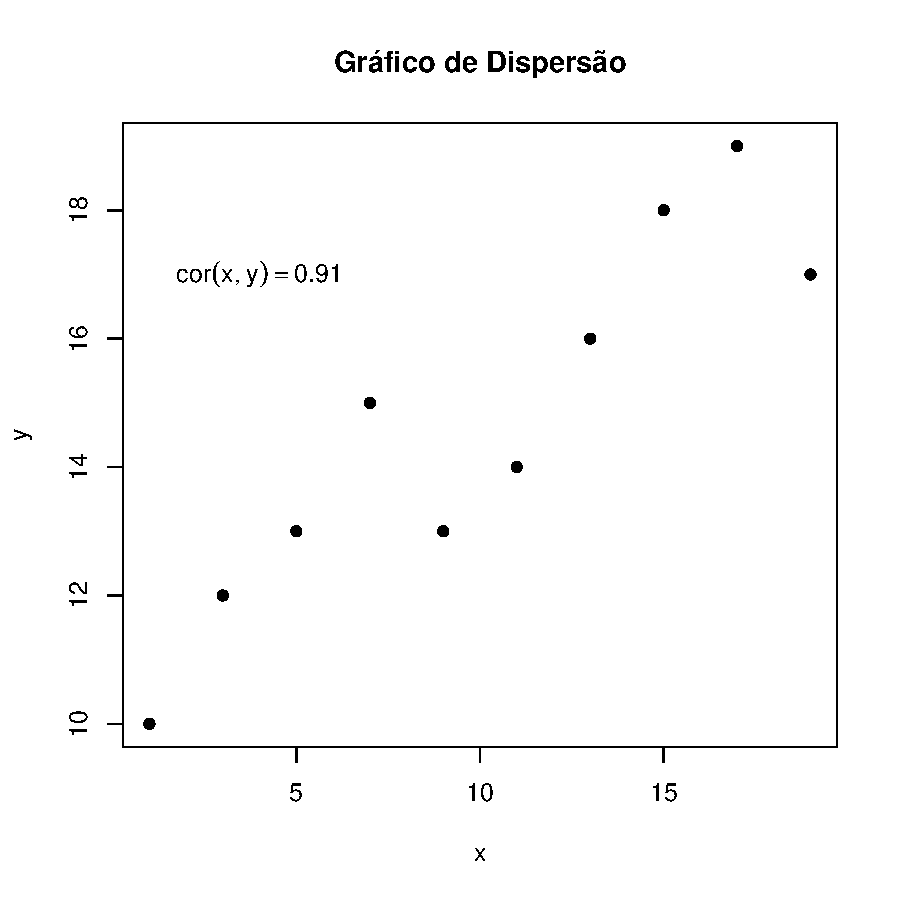
\includegraphics{Aula10-003}
\end{center}
\end{frame}

\begin{frame}[fragile]{}
\begin{center}
\setkeys{Gin}{width=0.6\linewidth}
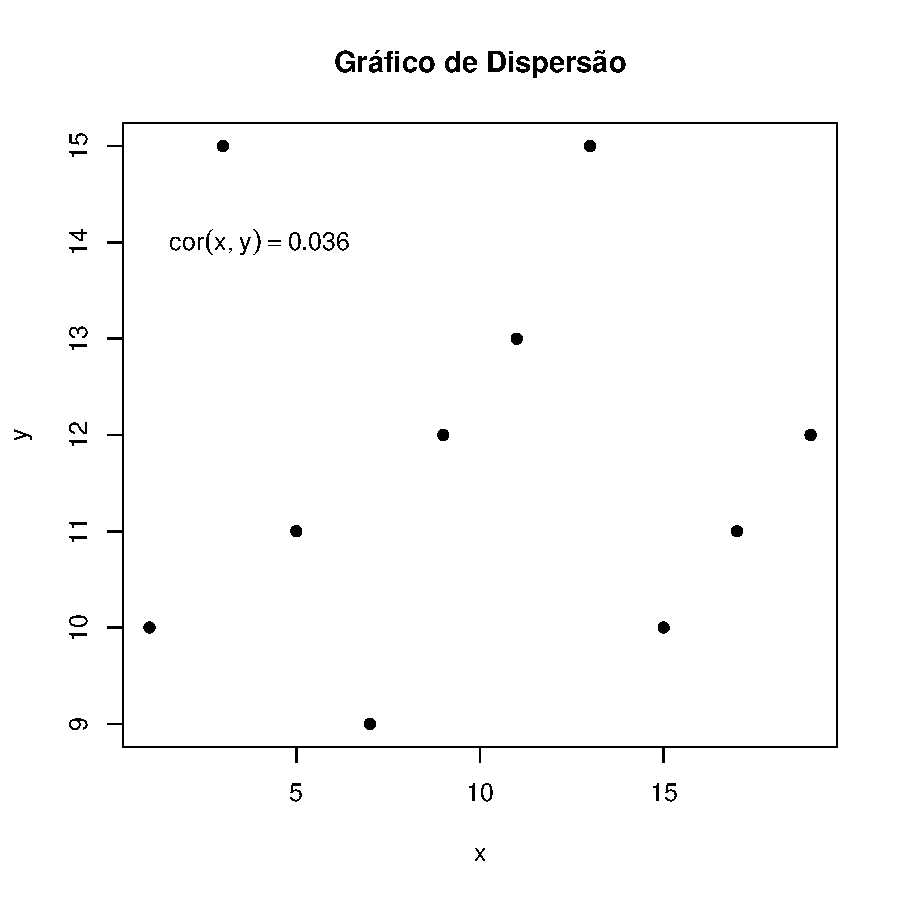
\includegraphics{Aula10-004}
\end{center}
\end{frame}

\begin{frame}[fragile]{}
\begin{center}
\setkeys{Gin}{width=0.6\linewidth}
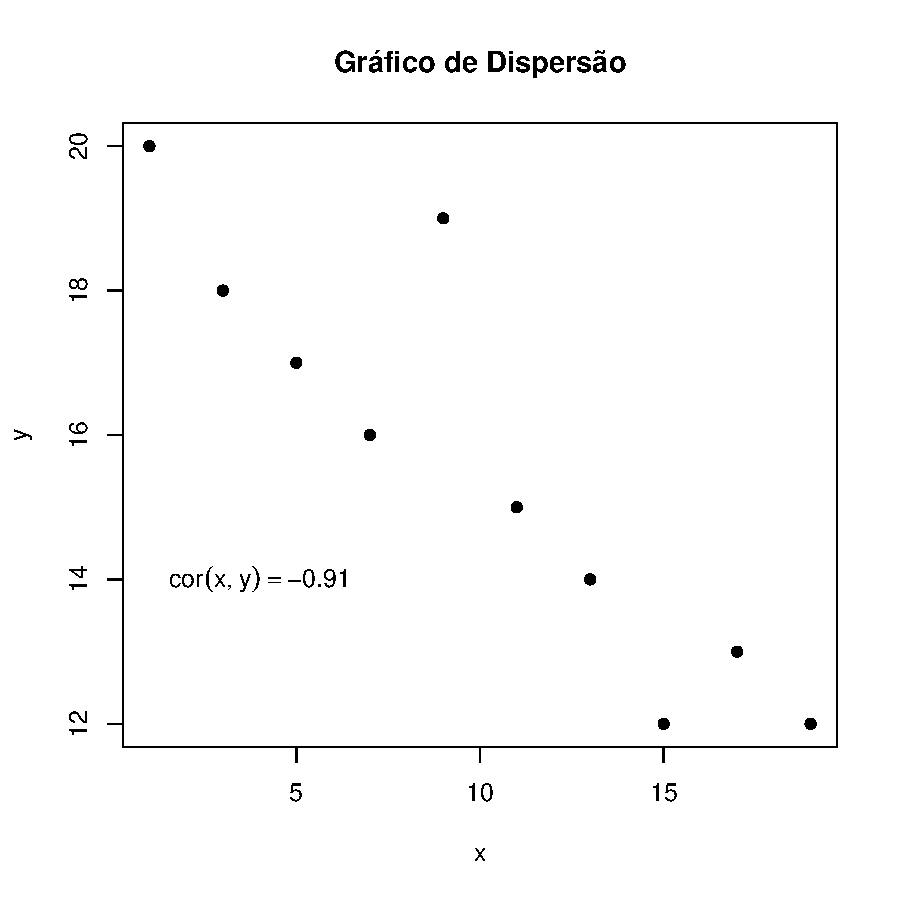
\includegraphics{Aula10-005}
\end{center}
\end{frame}

\begin{frame}[fragile]{}
\begin{center}
\setkeys{Gin}{width=0.6\linewidth}
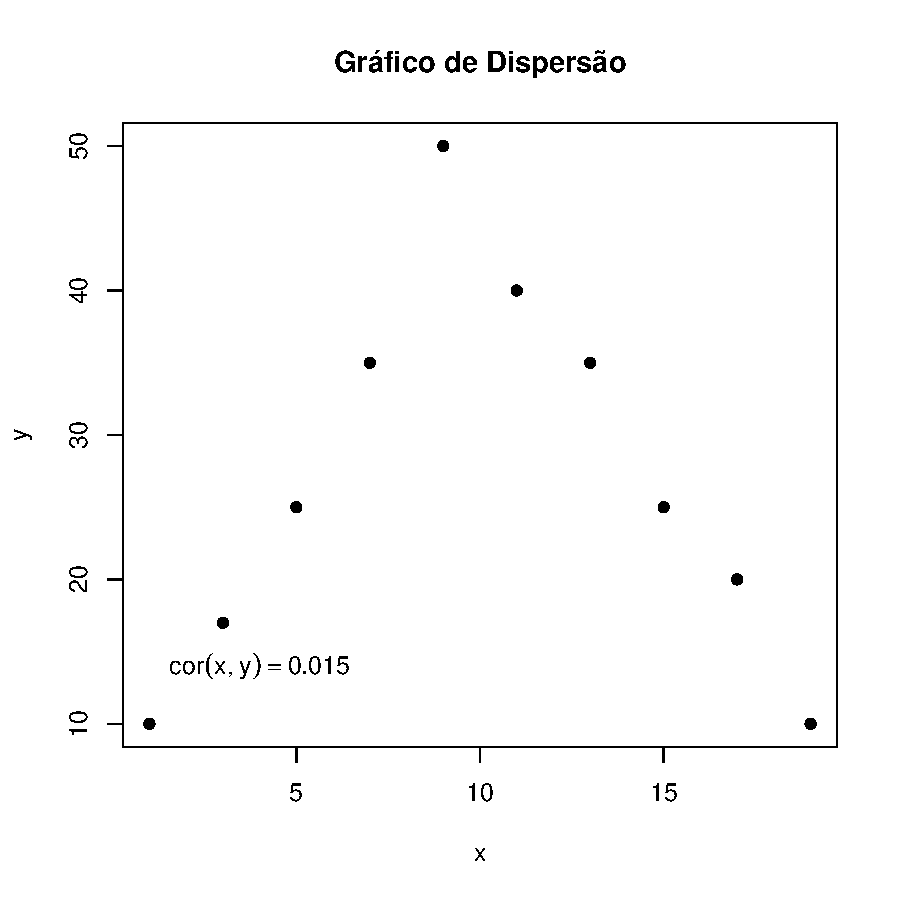
\includegraphics{Aula10-006}
\end{center}
\end{frame}

\begin{frame}{}
\frametitle{}
\vspace{-0.5cm}
% Table generated by Excel2LaTeX from sheet 'Plan1'
\begin{table}[htbp]
  \centering
  \caption{Cálculo do coeficiente de correlação.}
  \resizebox*{0.8\textwidth}{!}{%
    \begin{tabular}{c|c|c|c|c|c|c|c}
    \hline
    Agente & Anos  & Clientes & $x-\bar{x}$ & $y-\bar{y}$ & $\dfrac{x-\bar{x}}{dp(x)}=z_{x}$ & $\dfrac{y-\bar{y}}{dp(y)}=z_{y}$ & $z_{x}.z_{y}$ \\
    \hline
    A     & 2     & 48    & -3.7  & -8.5  & -1.54 & -1.05 & 1.617 \\
    B     & 3     & 50    & -2.7  & -6.5  & -1.12 & -0.8  & 0.896 \\
    C     & 4     & 56    & -1.7  & -0.5  & -0.71 & -0.06 & 0.043 \\
    D     & 5     & 52    & -0.7  & -4.5  & -0.29 & -0.55 & 0.160 \\
    E     & 4     & 43    & -1.7  & -13.5 & -0.71 & -1.66 & 1.179 \\
    F     & 6     & 60    & 0.3   & 3.5   & 0.12  & 0.43  & 0.052 \\
    G     & 7     & 62    & 1.3   & 5.5   & 0.54  & 0.68  & 0.367 \\
    H     & 8     & 58    & 2.3   & 1.5   & 0.95  & 0.18  & 0.171 \\
    I     & 8     & 64    & 2.3   & 7.5   & 0.95  & 0.92  & 0.874 \\
    J     & 10    & 72    & 4.3   & 15.5  & 1.78  & 1.91  & 3.400 \\
    \hline
    Total & 57    & 565   & 0     & 0     &       &       & 8.759 \\
    \hline
    \end{tabular}%
  \label{tab:addlabel}%
}
\end{table}%
$$Cor={\displaystyle \dfrac{1}{n}\sum_{i=1}^{n}\Biggl(\dfrac{x_{i}-\bar{x}}{dp(X)}\Biggl)\Biggl(\dfrac{y_{i}-\bar{y}}{dp(Y)}\Biggl)}=\dfrac{8.759}{10}=0.8759$$
\end{frame}

\begin{frame}{}
\frametitle{}
\vspace{-0.6cm}
\begin{block}{}
\justifying
Não é difícil provar que o coeficiente de correlação satisfaz:
$$-1\leq cor(X,Y)\leq 1$$
\end{block}
\pause
%\vspace{-0.8cm}
\begin{block}{}
\justifying
{\bf DEF:} Dados $n$ pares de valores $(x_{1}, y_{1}), \cdots, (x_{n}, y_{n}),$ chamaremos de covariância entre as duas variáveis $X$ e $Y$ a igualdade:
$$cov(X,Y)={\displaystyle \sum_{i=1}^{n}\dfrac{(x_{i}-\bar{x})(y_{i}-\bar{y})}{n}}$$
\end{block}
\pause
\vspace{-0.8cm}
\begin{block}{}
\justifying
Com a definição acima, o coeficiente de correlação pode ser escrito como:
$$cor(X,Y)=\dfrac{cov(X,Y)}{dp(X)dp(Y)}$$
\end{block}
\end{frame}

\begin{frame}{}
\frametitle{}
A covariância mede a relação linear entre duas variáveis. A covariância é semelhante à correlação entre duas variáveis, no entanto, elas diferem nas seguintes maneiras:
\begin{itemize}
\item Os coeficientes de correlação são padronizados. Assim, um relacionamento linear perfeito resulta em um coeficiente de correlação 1. A correlação mede tanto a força como a direção da relação linear entre duas variáveis.\pause
\item Os valores de covariância não são padronizados. Como os dados não são padronizadas, é difícil determinar a força da relação entre as variáveis.
\end{itemize}
\end{frame}

\section{Associação entre Variáveis Qualitativas e Quantitativas}
\begin{frame}{}
\frametitle{}
Associação entre Variáveis Qualitativas e Quantitativas
\begin{figure}[H]
    \centering
\begin{tikzpicture}[scale=0.5]
%\node {\includegraphics{boxplot.jpg}};
\draw[fill=black, line width=0.5mm] (-4.4,-1.4)--(-4.4,-3)--(-2.9,-3)--(-2.9,-1.4)--cycle;
\draw[white, line width=1mm] (-4.5,-2.4)--(-2.8,-2.4);
\draw[black, dashed, line width=0.5mm](-3.6,-3.1)--(-3.6,-3.8);
\draw[black, dashed, line width=0.5mm](-3.6,-1.3)--(-3.6,0.5);
\draw[black, line width=0.5mm] (-4.4,0.3)--(-4.4,0.5)--(-2.9,0.5)--(-2.9,0.3);
\draw[black, line width=0.5mm] (-4.4,-3.5)--(-4.4,-3.8)--(-2.9,-3.8)--(-2.9,-3.5);

\draw[fill=black, line width=0.5mm] (-0.2,0.9)--(-0.2,-1.7)--(1.3,-1.7)--(1.3,0.9)--cycle;
\draw[white, line width=1mm] (-0.3,-0.7)--(1.4,-0.7);
\draw[black, dashed, line width=0.5mm](0.5,-1.7)--(0.5,-2.9);
\draw[black, dashed, line width=0.5mm](0.5,0.9)--(0.5,2.8);
\draw[black, line width=0.5mm] (-0.3,2.7)--(-0.3,2.9)--(1.2,2.9)--(1.2,2.7);
\draw[black, line width=0.5mm] (-0.3,-2.7)--(-0.3,-2.9)--(1.3,-2.9)--(1.3,-2.7);

\draw[fill=black, line width=0.5mm] (3.9,2.6)--(3.9,0)--(5.4,0)--(5.4,2.6)--cycle;
\draw[white, line width=1mm] (3.8,1.8)--(5.5,1.8);
\draw[black, dashed, line width=0.5mm](4.6,0)--(4.6,-1);
\draw[black, dashed, line width=0.5mm](4.6,2.6)--(4.6,4.5);
\draw[black, line width=0.5mm] (3.9,-0.7)--(3.9,-1)--(5.3,-1)--(5.3,-0.7);
\draw[black, line width=0.5mm] (3.9,4.2)--(3.9,4.5)--(5.4,4.5)--(5.4,4.2);

\draw[black, line width=0.5mm, <->] (-6.8,6)--(-6.8,-4)--(7.7,-4); 
\node[black, line width=0.5mm] at (-7.7,3.1) {\small{20}};
\node[black, line width=0.5mm] at (-7.7,0.9) {\small{15}};
\node[black, line width=0.5mm] at (-7.7,-1.1) {\small{10}};
\node[black, line width=0.5mm] at (-7.4,-3.3) {\small{5}};
\node[black, line width=0.5mm] at (-3.6,-4.6) {\small{Fundamental}};
\node[black, line width=0.5mm] at (0.5,-4.6) {\small{Médio}};
\node[black, line width=0.5mm] at (4.6,-4.6) {\small{Superior}};
\draw[black, line width=0.5mm](-7,-3.3)--(-6.8,-3.3);
\draw[black, line width=0.5mm](-7,-1.2)--(-6.8,-1.2);
\draw[black, line width=0.5mm](-7,1)--(-6.8,1);
\draw[black, line width=0.5mm](-7,3.1)--(-6.8,3.1);

\end{tikzpicture}

    \caption{Box plots de salário segundo grau de instrução. \cite{Morettin09}}
    %\label{figRotulo}
  \end{figure}
\end{frame}

\begin{frame}{}
\frametitle{}
\begin{figure}[H]
    \centering
    \begin{tikzpicture}[scale=0.5]
%\node {\includegraphics{boxplot2.jpg}};
\draw[fill=black, line width=0.5mm] (-4,1.7)--(-4,-2.2)--(-2.6,-2.2)--(-2.6,1.7)--cycle;
\draw[white, line width=1mm] (-4.1,-1.3)--(-2.5,-1.3);
\draw[black, dashed, line width=0.5mm](-3.3,-2.2)--(-3.3,-3.3);
\draw[black, dashed, line width=0.5mm](-3.3,1.7)--(-3.3,2.6);
\draw[black, line width=0.5mm] (-4,-3)--(-4,-3.3)--(-2.6,-3.3)--(-2.6,-3);
\draw[black, line width=0.5mm] (-4,2.3)--(-4,2.6)--(-2.6,2.6)--(-2.6,2.3);

\draw[fill=black, line width=0.5mm] (-0.2,0.8)--(-0.2,-2.2)--(1.3,-2.2)--(1.3,0.8)--cycle;
\draw[white, line width=1mm] (-0.3,-0.9)--(1.4,-0.9);
\draw[black, dashed, line width=0.5mm](0.6,-2.2)--(0.6,-3.5);
\draw[black, dashed, line width=0.5mm](0.6,0.9)--(0.6,4.1);
\draw[black, line width=0.5mm] (-0.2,3.9)--(-0.2,4.1)--(1.3,4.1)--(1.3,3.9);
\draw[black, line width=0.5mm] (-0.2,-3.4)--(-0.2,-3.6)--(1.3,-3.6)--(1.3,-3.4);

\draw[fill=black, line width=0.5mm] (3.7,0)--(3.7,-1.6)--(5.1,-1.6)--(5.1,0)--cycle;
\draw[white, line width=1mm] (3.6,-1.2)--(5.2,-1.2);
\draw[black, dashed, line width=0.5mm](4.4,-1.6)--(4.4,-2.9);
\draw[black, dashed, line width=0.5mm](4.4,0)--(4.4,1.3);
\draw[black, line width=0.5mm] (3.7,-2.8)--(3.7,-2.9)--(5.2,-2.9)--(5.2,-2.8);
\draw[black, line width=0.5mm] (3.7,1.2)--(3.7,1.4)--(5.2,1.4)--(5.2,1.2);

\draw[black, line width=0.5mm, <->] (-6.1,5)--(-6.1,-4)--(7.7,-4); 
\node[black, line width=0.5mm] at (-6.8,3) {\small{20}};
\node[black, line width=0.5mm] at (-6.8,0.9) {\small{15}};
\node[black, line width=0.5mm] at (-6.8,-1.1) {\small{10}};
\node[black, line width=0.5mm] at (-6.8,-3.1) {\small{5}};
\node[black, line width=0.5mm] at (-3.6,-4.5) {\small{Capital}};
\node[black, line width=0.5mm] at (0.5,-4.5) {\small{Interior}};
\node[black, line width=0.5mm] at (4.6,-4.5) {\small{Outra}};

\draw[black, line width=0.5mm](-6.4,-3.2)--(-6.1,-3.2);
\draw[black, line width=0.5mm](-6.4,-1.2)--(-6.1,-1.2);
\draw[black, line width=0.5mm](-6.4,0.9)--(-6.1,0.9);
\draw[black, line width=0.5mm](-6.4,2.9)--(-6.1,2.9);
\end{tikzpicture}
    \caption{Box plots de salário segundo região de procedência. \cite{Morettin09}}
    %\label{figRotulo}
  \end{figure}
\end{frame}

\begin{frame}%[allowframebreaks]
\frametitle{\bf Referências}
\bibliography{Referencias.bib}
\end{frame}


\end{document}
